\section{Data Preparation}

\subsection{What was your data source?}

Three datasets were used in this analysis.

The first, as noted above, was the Government of Canada's Open Government Portal~\cite{ogp}.
The name of the dataset is NAFO Division 4T groundfish research vessel trawl survey (September Survey) dataset~\cite{groundfish}.
The dataset contained information ecological information (i.e., species caught, specimen counts and specimen weights),
fishing information (i.e., gear type used, fishing vessel) and spatial information (i.e., latitude and longitude).
For mapping purposes, I also used a geospatial file of the Canada Provincial Boundaries from the same catalogue~\cite{canmap}.

The dataset did not contain and elevation data and therefore this had to be acquired elsewhere.
Luckily, there is an excellent website and web app called the General bathymetric Chart of the Oceans (GEBCO),
which is maintained by the international community~\cite{gebco}.
The web app provides an interface for downloading world ocean's bathymetric data.

\subsection{How good was the data quality?}

The quality of the fishing data was excellent.
There were no missing values and the column data types were respected.
For example, the columns that you would expect to be \textit{float} type, e.g., lat/lon values, were indeed.
The dataset was accompanied by a data dictionary, which contained clear explanation of the variables in both English and French.
The only thing worth mentioning was that the coordinate reference system for the latitudes and longitudes were difficult to obtain.
They are not displayed on the website but the metadata XML file did specify EPSG 4269.

\subsection{What did you need to do to procure it?}

The data from the Open Government Portal was downloaded using a web browser.
The data was accessible via a static link.
The format of the fishing data was a single comma separated values (CSV) document and the map was formatted as a GEOJSON file.
The GEBCO elevation data was downloaded using their customizable web application.
In this application, I was able to download the bathymetric data as a NetCDF file for only the area of interest.
I was very impressed with this tool!


\subsection{What tools or code did you need to use to prepare it for analysis?}


\subsubsection{Fishing Data}

As noted above, the species / fishing data was very clean.
I loaded the data from its original CSV into a pandas dataframe.
I ensured all the data types made sense using the \textbf{DataFrame.info()} method.
The dataset contained 166,694 rows of data; each one being a species observation at a particular place and time.
When exploring the dataset, it became apparent that these for a given coordinate on a given date, there were many species observed.
For the sake of efficiency, I parsed the original dataset into two separate dataframes:
one containing the biological information (species observed, how many, total weight)
and the other containing the site / fishing set details (time, date, lat/lon).
The linkage between the two tables was made by a fishing set ID column (\textbf{site\_id}).
After this was done, I was dealing with a total of 7,257 fishing sets which can be seen in Figure~\ref{fig:set_map}.


\subsubsection{Mapping Data}

The GEOJSON file was loaded using the geopandas python library into a geodataframe.
The only data preparation needed for these data was to reproject the dataset to the same coordinate reference system as the fishing data.
As noted above, the point data from fishing was presented in EPSG 4269.
Without this step, the points and polygons cannot be represented on the same map.


\subsubsection{Elevation Data}

The elevation data was downloaded in NetCDF format and loaded directly into the python Xarray library~\cite{xarray}.
When plotted using \textbf{Matplotlib}, you can clearly see the familiar contours of Atlantic Canada, the characteristic
shallow waters of the sGSL and the deeper waters out in the channel of the St. Lawrence seaway (see Figure~\ref{fig:elevation_map}).

Using this two-dimensional array of elevation data, the next step was to extrapolate an elevation value for each fishing set in the fishing set dataframe.
To do this, I followed an example from the \textbf{Xarray} docs.
Specifically, I made use of the Data Array \textit{sel} method.
This method has an argument called \textit{method} which specifies how to deal with inexact matches, i.e.,
when trying to determine elevation for a set of coordinates that are not in the array. I decided to use the \textit{nearest} method,
which returns value from the nearest coordinate.

# use the "nearest" method to determine how to deal with the miss elevation value for this coordinate pair

We wanted elevation for each point of the fishing dataset


QC of checking that no sites had an elevation > 0






\subsection{What challenges did you face?}

Since geographic information systems is not my area of expertise, I found it challenging figuring out how to reproject a geographical data to another
coordinate reference system.
In the end, this was not too difficult, but it took time to figure out.

Another major challenge was learning about the Xarray python package~\cite{xarray}.
This is a very impressive package, albeit quite complex.
It took me a long time to figure out how to extract the data from a data array, manipulate it and create a new data array.


\begin{figure}
    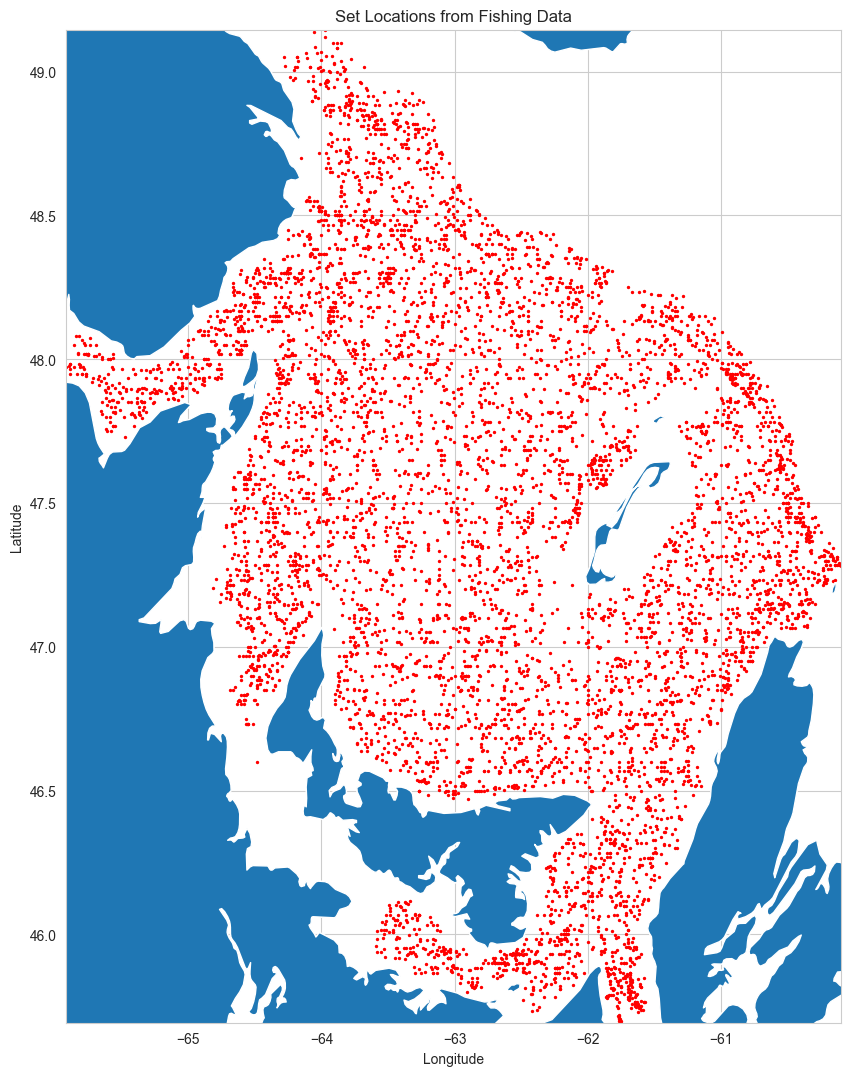
\includegraphics[width=\linewidth]{sites_map}
    \caption{This figure displays the 7,257 fishing sets contained in this dataset. A fishing set is represented by a red point.}
    \label{fig:set_map}
\end{figure}


\begin{figure}
    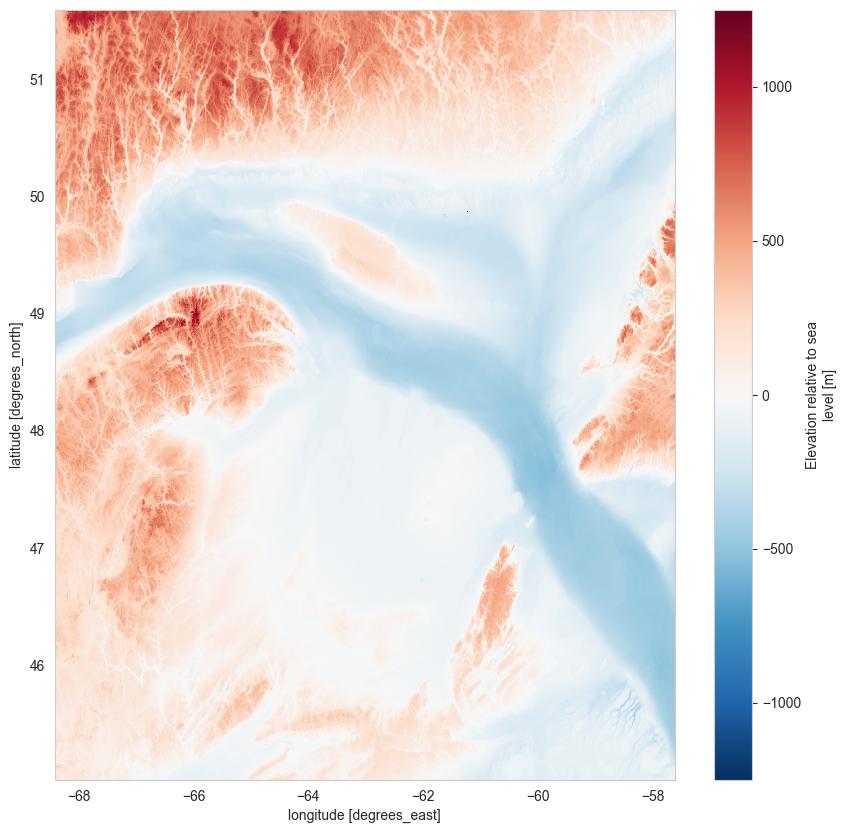
\includegraphics[width=\linewidth]{elevation_map}
    \caption{This figure shows the raw elevation data array. The values are color codes according to the elevation in meters}
    \label{fig:elevation_map}
\end{figure}
